%%%%%%%%%%%%%%%%%%%%%%%%%%%%%%%%%%%%%%%%%%%%%%%%%%%%%%%%%%%%%%%%%%% 
%                                                                 %
%                            CHAPTER ONE                          %
%                                                                 %
%%%%%%%%%%%%%%%%%%%%%%%%%%%%%%%%%%%%%%%%%%%%%%%%%%%%%%%%%%%%%%%%%%% 
 
\chapter{Introduction} \label{sec:introduction}
 
\section{Humpback Whales}

Since the international ban on commercial hunting of Humpback whales in 1966, humpback whales have grown from a population of only 5000 \cite{baker1993abundant} to over 50000 \cite{branch2011humpback}. 
As the population grows, it becomes more and more important to be able to automatically identify individual whales in order to accurately monitor their population growth and follow their migration patterns, among other ecological conservation endeavours.
One of the most reliable methods for photo-identifying humpback whales is by taking pictures of their flukes as they dive after breaching the surface of the water.

\begin{figure*}[t]%
\centering
\subfloat[][Individual ID: 420223]{
	\includegraphics[width=0.5\textwidth]{../images/results/aid88_nid47.png}
}
\subfloat[][Individual ID: 470601]{
	\includegraphics[width=0.5\textwidth]{../images/results/aid863_nid489.png}
}
\newline
\subfloat[][Individual ID: 420223]{
	\includegraphics[width=0.5\textwidth]{../images/results/aid87_nid47.png}
}
\subfloat[][Individual ID: 470601]{
	\includegraphics[width=0.5\textwidth]{../images/results/aid864_nid489.png}
}
\caption{\textbf{Example Flukes}. Example images of humpback whale flukes from the SPLASH \cite{calambokidis2008splash} dataset. These flukes both have distinctive internal textures (more so on the left). However, the trailing edge on the left is far more distinctive than the trailing edge on the right.}
\label{fig:example_fluke}
\end{figure*}

\subsection{Distinguishing Individual Flukes}

The primary distinguishing features of these flukes are --- for the purposes of this work --- separated into two main areas; the ``trailing edge'' of the fluke, and the internal texture (see Figure \ref{fig:example_fluke}).
%There are pros and cons to identification with either feature.
The internal texture is a more obvious choice for identification, as it is disinctive even from a distance even when the image is blurred.
%whereas trailing edges require high quality photographs.
Unfortunately, some humpback flukes have indistinct (e.g.\ all-black) internal textures, which make matching based on texture impossible (see Figure \ref{fig:unclear_texture}).
Additionally, the work of Blackmer et al.\ \cite{blackmer2000temporal} finds that the trailing edge changes less with age than the internal texture of the fluke, which means that it can (potentially) be a more reliable identifier over time.
That said, the requirements for getting a good photograph of the trailing edge can be impractical, as the trailing edge is vulnerable to being obscured by out of plane rotations (see Figure \ref{fig:unclear_te}), and as such are optimally photographed when the fluke is ``flat'' to the photographer.


\section{Current Identification Methods}

Computer-assisted photo-identification of humpback whale flukes has been attempted since the early 90s \cite{mizroch1990computer}.
While early efforts mostly relied on a manual description of the fluke that would then be matched against other stored descriptions \cite{mizroch1990computer, whitehead1990computer}, later efforts have involved matching flukes based on automated analysis of both the internal texture and trailing edge \cite{hughes2015automated, kniest2010fluke, i3scontour}.
\\\\
Existing computer-assisted photo-identification methods can be broadly separated into three categories.
There are manual methods, in which humans both identify and describe distinguishing features, semi-automated methods, in which humans identify distinguishing features that are then described and matched automatically, and automated methods --- which can match based solely on raw images with no human involvement. 


%\begin{itemize}
%	\item Manually annotated -- a human must manually annotate or catalogue features on each fluke image, which are then automatically matched
%	\item Semi-automated -- a human must guide an algorithm (e.g.\ by setting control points or highlighting interesting regions) that then automatically identifies the individual
%	\item Fully-automated -- the algorithm can identify individuals from raw images
%\end{itemize}
\subsection{Based on Trailing Edge}

In the $\text{I}^3\text{S}$ contour system \cite{i3scontour}, the user must input start and end points on the query trailing edge, after which its contour is extracted.
This trailing edge is then resized and aligned so that it can be compared with absolute difference against the database trailing edges.
It also compares a set of possible shifts, rotations, and scales of the query trailing edge to account for these differences.
At the time of writing no published results on this system applied to humpback whales could be found.

Automatically identifying humpback whales by their entire trailing edge contour is done experimentally in Hughes et al.\ \cite{hughes2015automated}, using a technique that is originally designed for great white sharks. 
This technique segments the trailing edge into a set of possible contours and matches them combinatorially using Difference of Gaussians.
The authors achieve a comparable accuracy to our method, however for a much smaller dataset of humpback flukes than the one evaluated here.

\begin{figure*}[t]%
\centering
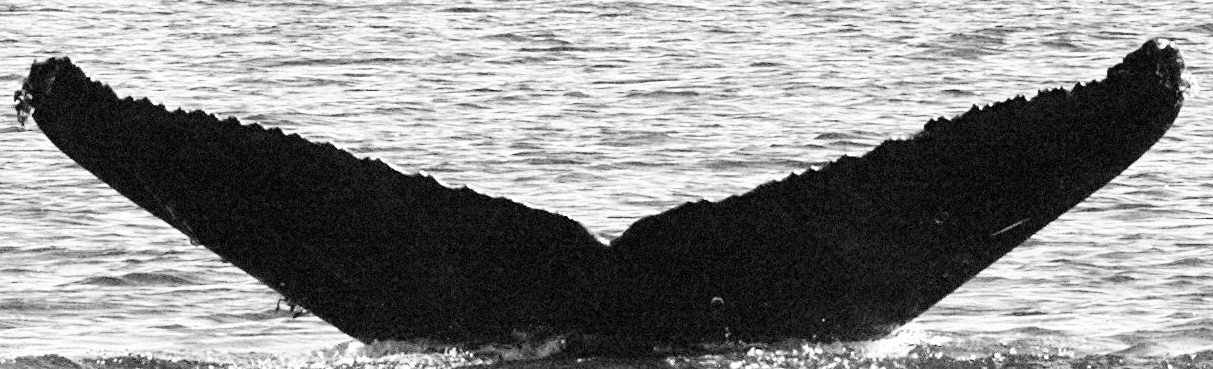
\includegraphics[width=1.0\textwidth]{../images/unclear_texture.jpg}
\caption{\textbf{Uniform Internal Texture}. This image of a humpback fluke shows no clear internal texture, but a distinctive trailing edge.}
\label{fig:unclear_texture}
\end{figure*}

While trailing edge matching has seen limited use in humpback whale identification, it is a much more common technique in sperm whale (P.\ macrocephalus) identification \cite{huele2000finding, beekmans2005comparison, whitehead1990computer} --- with varying levels of manual effort.
%We detail these methods below as the fluke trailing edge matching paradigm is similar across species.
In Whitehead's work \cite{whitehead1990computer}, points of interest on the trailing edge are entered and catalogued manually along with their positions.
In order to match these trailing edges, all of the points are compared against points on annotated trailing edges in the database, using a distance threshold to ensure locality.
This is a manual method, requiring extensive annotation for matching.

The method proposed by Huele et al.\ \cite{huele2000finding} uses a semi-automatic extraction of sperm whale trailing edge, and then applies wavelet transformations which are cross-correlated to determine a similarity measurement.

An investigation of the above methods for sperm whale identification is carried out in the work of Beekmans et al.\ \cite{beekmans2005comparison}, showing that combining these two methods yields an 80\% top-1 accuracy (meaning that the correct identity is ranked at the top of the potential matches 82\% of the time) on a slightly smaller dataset than ours.
However on their own each method only achieves about 65\% top-1 accuracy.

\begin{figure*}[t]%
\centering
\subfloat[][]{
	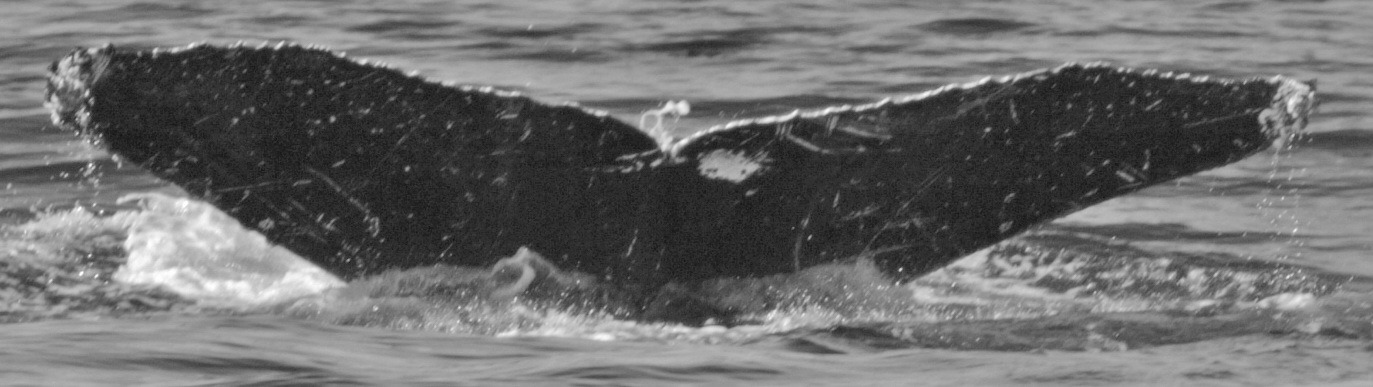
\includegraphics[width=1.0\textwidth]{../images/unclear_te_q.jpg}
}
\newline
\subfloat[][]{
	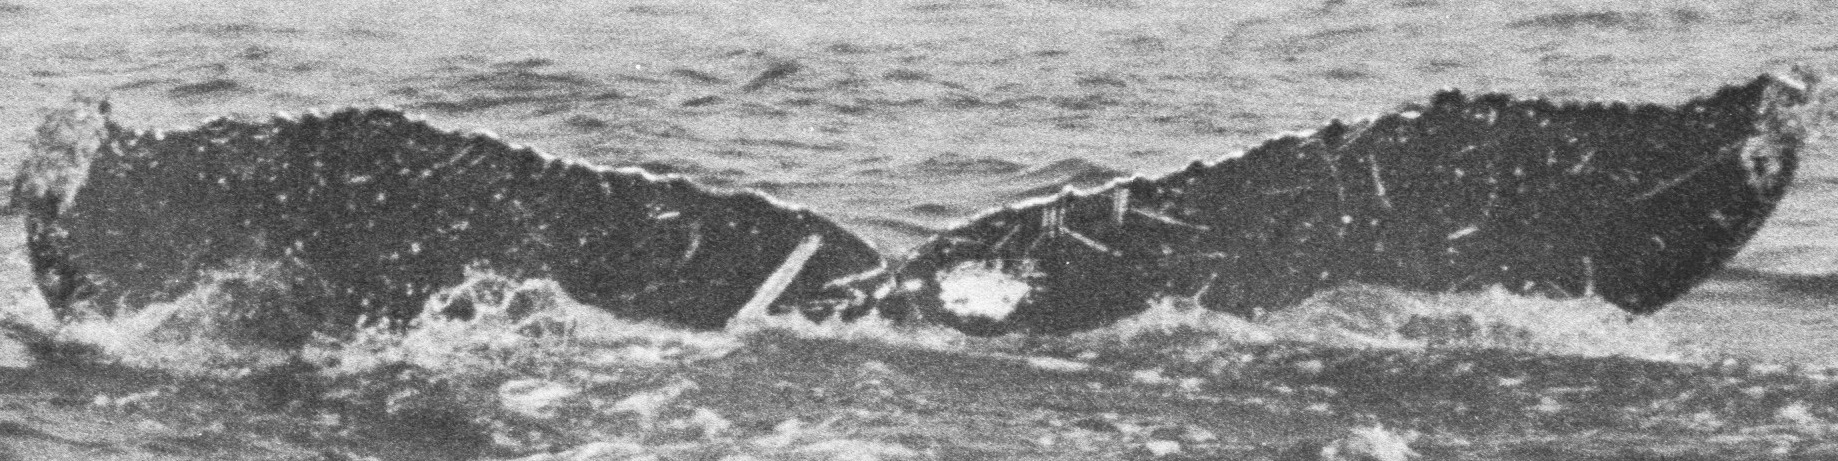
\includegraphics[width=1.0\textwidth]{../images/unclear_te_gt.jpg}
}
\caption{\textbf{Change in Trailing Edge}. The above images show that out of plane rotations of the fluke can obscure it or otherwise make it hard to match. These images are both of the same individual, however in the top image the fluke is rotated slightly towards the camera.}
\label{fig:unclear_te}
\end{figure*}

\subsection{Based on General Fluke Appearance}


The primary paradigm for computer-assisted photo-identification of humpback whale flukes is to use the internal fluke pattern, as seen in the work of Mizroch et al.\ \cite{mizroch1990computer} and the Flukematcher \cite{kniest2010fluke} of Kniest et al\footnote{Flukematcher also uses information about the trailing edge, but is focused on the internal fluke texture}. 

In Mizroch et al., information about the fluke is manually catalogued and used to match individual whales. 
The fields that are catalogued contain information primarily about the overall coloration patterns of the fluke, as well as the shape of the central notch. 
The matching algorithm generates potential fluke matches by looking at how similar the annotated patterns are.
This requires significant manual effort to identify individuals.

In Flukematcher \cite{kniest2010fluke}, control points are manually annotated which allow the program to automatically find pigmentation patterns in the fluke and align accordingly.
Optionally, distinctive fluke patterns can also be selected and annotated by the user.
A variety of heuristic features are then extracted, which are matched using a variety of similarity measures.
This method has acheived a 82\% top-1 accuracy on a smaller dataset than ours.
However, it requires significant manual effort on the order of five minutes per fluke photograph.

\section{Method Outline}

% Short sentence about this

In this thesis, we develop and present an efficient fully-automated\footnote{With the caveat that manual annotation is needed to train parts of the algorithm} algorithm that identifies humpback flukes based on their trailing edges.
For each fluke, the algorithm first determines the left and right tip points of the fluke (as well as the bottom of the central notch). 
The trailing edge contour is then extracted between the left and right tip points (see Figure \ref{fig:example_overlay}), and for each point on this contour curvature is measured at multiple scales.
Once these curvatures are extracted for each fluke photograph, the algorithm computes the distance between a query fluke and possible identities by aligning its contour curvature against contour curvatures in the database and computing distance with dynamic time warping.
The query fluke is then given the identity of the database fluke with the lowest distance.
This method is based on both traditional edge detection and curvature techniques, modern machine learning, and classical fast sequence comparison.

%\begin{itemize}
%	\item Find the left and right tips of the fluke
%	\item Extract the trailing edge contour betweeen these points
%	\item Compute the curvature of the trailing edge contour at multiple scales
%	\item Determine a ranking of possible identities using a distance computed by dynamic time warping 
%\end{itemize}

\begin{figure*}[t]%
\centering
\includegraphics[width=1.0\textwidth]{../images/results/aid951_te_kp_overlay.png}
\caption{\textbf{Example Keypoint and Trailing Edge Annotation}. This image shows a typical set of fluke keypoints and trailing edge extracted by our algorithm.}
\label{fig:example_overlay}
\end{figure*}

We also show we can greatly improve the accuracy of this method by combining it with matches found by Hotspotter, a generalized pattern based identification method that is a powerful matching algorithm for several species \cite{crall_hotspotter_2013}.
Hotspotter extracts keypoints with SIFT descriptors in an image that are then spatially verified and matched with other keypoints in the database to produce a ranking over possible identities. 
Despite the general nature of this method, we find that it does not identify keypoints on the trailing edge and thus struggles with flukes that have no significant internal texture. 
This work is the first to our knowledge that details Hotspotters efficacy when applied to humpback whale flukes, and the results are presented in Chapter 4.
%It should be noted that we used a segmenting convolutional network to aid Hotspotter's predictions, although this is not detailed in this work.

\section{The Dataset}

The main dataset that is used and evaluated in this work is a subset of the dataset collected by the SPLASH project \cite{calambokidis2008splash}. 
It consists of about 1400 identified photographs spread over about 860 identified individuals.
Of these, only 433 individuals have more than one image associated with them, giving 942 images that can be used in a one-to-one comparison.
We refer to this dataset as the Flukebook dataset, which is the team from which it originates.
All images shown in this thesis come from this dataset.

Additionally, an external dataset of unidentified (but annotated) humpback flukes is used for training individual components of the method.


\section{Thesis Outline}

% Main body background in chapter 2
% Primary method in chapter 3, as well as a brief description of some of the alternative methods that were tried
% Reesults presented in chapter 4
% Discussion and future work presented in chapter 5

The rest of this thesis starts by giving a background on the algorithms that our method is based on in Chapter \ref{sec:background}.
Afterwards, the main method is detailed in Chapter \ref{sec:methods}, along with a description of some alternate methods that failed to work as well.
Chapter \ref{sec:results} goes into the results of the primary algorithm as well as various configuration changes and how they affect the results.
We also describe the effectiveness of this identification method in combination with Hotspotter.
This thesis concludes with a discussion on the failings of the primary method, as well as ways to improve it and generalize it to extracting and matching edge characteristics in other animals.

The primary contributions of this work are the individual components of the main method for extracting trailing edges and fluke keypoints, as well as the combination of all the components into a coherent identification pipeline.
We also contribute an evaluation of dynamic time warping on curvature measures as a method for matching humpback flukes, as well as an evaluation of Hotspotter for this task.



% Contributions
% A convolutional network and loss for extracting fluke keypoints
% A simple trailing edge extractor for humpback flukes
% A convolutional network for predicting where the trailing edge is
% Curvature extraction and matching algorithm



%\section{Method Overview}

%The method for trailing edge identification put forth in this thesis is very nearly fully automated, requiring no human annotation when used (although manual annotation is necessary for training the machine learning models used).
%On its own, it achieves decent results on a (relatively) large dataset, comparable with the fully automated method used in \cite{hughes2015automated}. 
%Ultimately we find that this method is best used in combination with an automated pattern matching method (e.g. Hotspotter) to provide high accuracy matches.
%We also explore alternative methods based on more recent advances in deep learning for identification, however it appears that the dataset is too small to properly train these methods.


%%% Local Variables: 
%%% mode: latex
%%% TeX-master: t
%%% End: 
